\documentclass[11pt]{article}
\usepackage{geometry}                % See geometry.pdf to learn the layout options. There are lots.
\geometry{a4paper}                   % ... or a4paper or a5paper or ... 
%\geometry{landscape}                % Activate for for rotated page geometry
\usepackage[parfill]{parskip}    % Activate to begin paragraphs with an empty line rather than an indent
\usepackage{graphicx}
\usepackage{amssymb}
\usepackage{epstopdf}
\DeclareGraphicsRule{.tif}{png}{.png}{`convert #1 `dirname #1`/`basename #1 .tif`.png}

\title{Overview of Repository as a Service WSDL Generation from Ecore Models}
\author{Keith Duddy and J\"org Kiegeland\\QUT}
\date{17 May 2011}                                           % Activate to display a given date or no date

\begin{document}
\maketitle
\section{Introduction}
This document provides an overview of the WSDL interfaces generated from Ecore models by the Repository as a Service code generator. It explains the WSDL operations and their semantics as a pattern based on the classes in the Ecore models used as input, and the XML types generated for use as parameters to these operations.

A Simple Ecore model that contains just enough structure to demonstrate the code generation principles and patterns is used throughout this document. It is known as ``small\_test.ecore'', and is shown in Figure \ref{small-test}. Ecore Annotations are shown as yellow ``sticky notes'' attached to model elements.

\begin{figure}[htbp]
\begin{center}
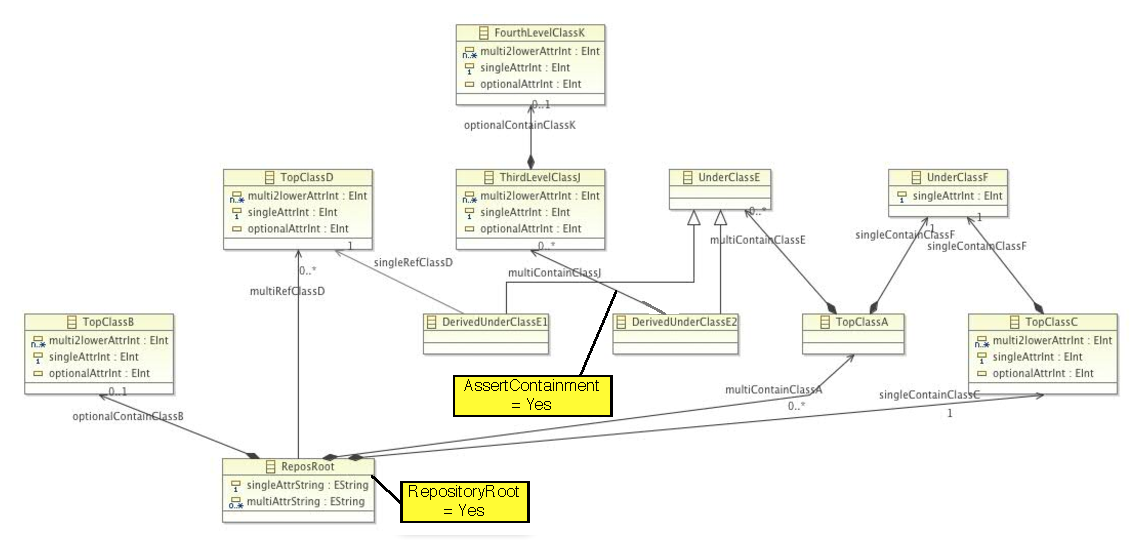
\includegraphics[width=15cm]{SmallTestEcoreWithAnnotations.pdf}
\caption{The small\_test Ecore model}
\label{small-test}
\end{center}
\end{figure}

\section{Primary Concepts in Repository Generation} \label{primary-concepts}

\subsection{Ecore}
Ecore models suitable for repository specifications are a simple subset of UML that has five main concepts for representing object oriented metadata designs:
\begin{description}
\item[Package] A container for the other Ecore concepts which is a namespace for its contents. Packages are not usually shown in Ecore diagrams, but all other model elements must be contained in a package.
\item[Class] A specification for a set of object instances. Classes are shown as boxes with their name in the top compartment and attributes in the next compartment. Classes may specialise (or inherit from) other classes, which is shown as an arrow with a white triangular head. 
\item[Attribute] A data value contained by a Class of some DataType which must be a simple type such as Strings, Integers, or Enumerated Values. Attributes have multiplicities which state how many values an object may/must contain in terms of a lower bound and an upper bound. A zero lower bound makes a value optional, and an asterisk for an upper bound means any number of values may be contained.
\item[Reference] A ``'pointer'' from one class to another which has a name, a multiplicity (which states how many references an instance of the class may/must hold) and a containment indicator (shown as a black diamond, which indicates that the object referred to is owned or contained by the referencing object, and when the owner is destroyed, all of its contained objects are also destroyed).
\item[Annotation] A textual name/value pair that is attached to some Ecore model element to allow specifiers to ``mark up'' their models with arbitrary additional information.
\end{description}

Ecore also supports operations on classes, but we do not use this feature, as the models for input to Repository generation are data-only models. The presence of operations is simply ignored at the moment. 

Enumerations {\em are} supported in Repository generation, and may be used as attribute types. We do not show their use in the small test model. 

The Eclipse Modelling Framework (EMF) maps Ecore models to Java code, in a very simple way, generating the Java code framework automatically, including support for serialisation and tree-based editors.  Ecore packages map to Java packages, enumerations to enumerations, classes to classes, attributes to attributes, and references to object-valued attributes (pointers).

\subsection{Patterns for Code Generation}

The primary goal of generating a Web services wrapper around an EMF-based data store is to change the access pattern for distributed programs from being based on getter and setter operations for each individual attribute and reference of a class, to a medium-granularity model where a set of objects linked via containment references are serialised as an XML structure, and the whole sub-tree of the model can be created, retrieved, updated or deleted (c.f. ``CRUD''\footnote{$http://en.wikipedia.org/wiki/Create,\_read,\_update\_and\_delete$}) with a single WSDL operation invocation.

The first repository-specific concept that we need to explain is the {\bf Repository Root}. This is a single class in the input Ecore model that is considered central to the repository. In the example model shown in Figure \ref{small-test} this class is called {\em ReposRoot}, and it is marked for the Repository code generator with an annotation ``RepositoryRoot=Yes''. This class is at the root of a tree of containment references (arrows with black diamonds at the ``container'', or source end of the reference).   A real-world example is the {\em Service} class of the USDL model, which was used extensively to test the concepts used for Repository building. There may be multiple classes nominated as repository root, however for each such repository root the code generator generates a custom web service, which are independent from each other (e.g. each web service has its own WSDL), so for simplicity we consider the web service generation for only one repository root. 

The repository root class is treated differently from other classes - and we will explain this below once it is understood how other classes are treated for code generation.

The next concept that we introduce is the notion of a {\bf Top Class}. Top classes are those classes which are not contained by another class via a containment reference {\em other than the repository root}. In Figure \ref{small-test-code} the top classes are shown with yellow stars (and are all named TopClass$X$ to assist with code generation inspection). 

Because we wish to generate repositories from standardised Ecore models, such as USDL, without needing to change these models, the concepts of an {\bf Asserted Containment} is introduced. This assertion is made by attaching an Ecore annotation ``AssertContainment'' to a reference that is not a containment (no black diamond), when the domain semantics of the model does not imply that the referenced class will ever need a lifecycle or re-use separate from the its use as a target of that reference. In  \ref{small-test-code} we make this assertion on the reference {\em multiContainClassJ}, and the code generators will treat this reference as if it is containment.

The reason why the repository root is not considered a top class is that in many metadata models this would mean that the tree of classes involved in its containment hierarchy would include almost every class in the model - and this would generate an extremely coarse-grained interaction with the repository, in which a serialisation of an instance of almost the whole model would be created and stored in the repository using a single WSDL operation invocation. Whereas the nomination of a repository root allows this class to be created without including all of its contained classes, and each containment reference from the repository root will form a sub-tree of classes for which instances can be added to the root class instances using operations generated for each subtree, which is headed by a top class. This means that ``aspects'' of the repository's main concept class can be populated one at a time, and that the granularity of interaction with the generated Web service is medium-grained, rather than very coarse-grained as would be the case if the repository root were considered to be a top class.

\begin{figure}[htbp]
\begin{center}
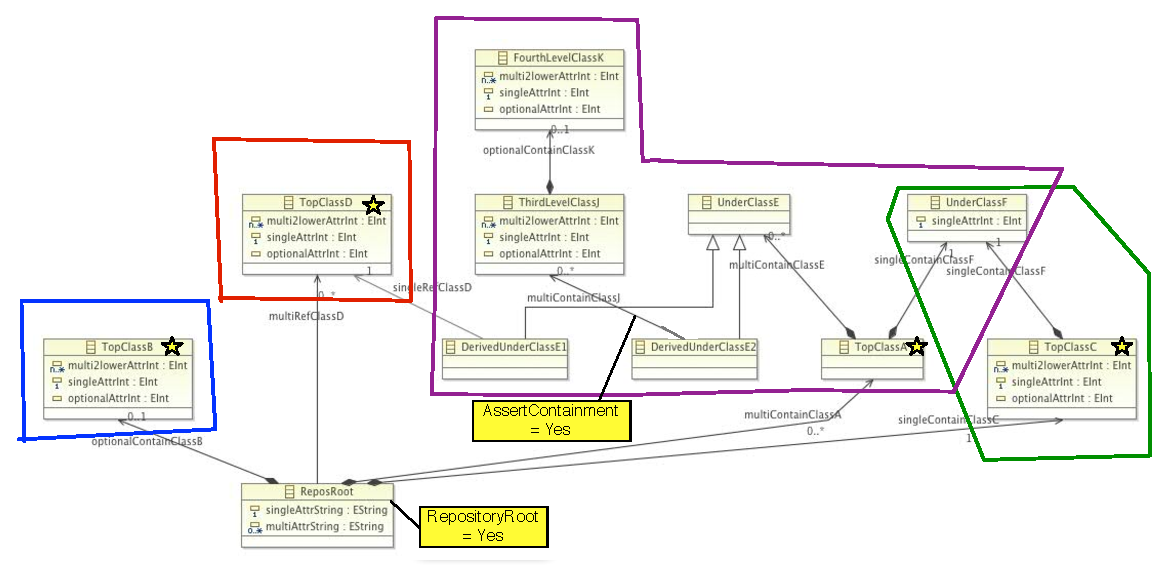
\includegraphics[width=15cm]{SmallTestEcoreWithCodeGen.pdf}
\caption{The small\_test Ecore model showing code generation}
\label{small-test-code}
\end{center}
\end{figure}

\section{Generated WSDL}

\subsection{WSDL and XML Basics}

WSDL is a very verbose language that forces separately named elements to be declared for operations as interfaces (in {\em portTypes}) and again for bindings of those operations into service implementations (in {\em bindings} and {\em service ports}). It also forces the operations' input parameters and return values to bundled into named {\em messages}, and for both the {\em operations} in the {\em portTypes} and {\em bindings} to make reference to these {\em messages}.

To avoid dealing with the complexity of WSDL, the RaaS code generator chooses the code-first approach in contrast to the WSDL-first approach.
This means that the generator basically generates Java code artefacts, and the WSDL is generated automatically from the Java code.
In fact, the WSDL is generated ``on demand'' when actually the RaaS repository deployed on a web server.

The generated WSDL will use the document/literal wrapped style over SOAP by default. As with many other aspects of automatic WSDL generation, this can be influenced by using JAXWS annotations applied to the generated Java classes and Java method signatures from EMF; in this case the {\em SOAPBinding} annotation. If the SOAPBinding annotation is not applied to the generated Web service implementation class, it defaults to following:
\begin{verbatim}
@SOAPBinding(style = SOAPBinding.Style.DOCUMENT, 
    use = SOAPBinding.Use.LITERAL, 
    parameterStyle = SOAPBinding.ParameterStyle.WRAPPED)
\end{verbatim}

\subsection{Simulating Object Orientation}

As WSDL is not object-oriented, and uses XML Schema as its type language for operation parameters and return values, we need to introduce some generated features into the WSDL and XML to allow the correct objects to be identified by clients of the repository.

Firstly, we introduce an additional attribute into the Ecore model for each class. This is called {\em raasRef} and is of type string. It is expected to contain a unique identifier, and when an object sub-tree is added to the repository, its allocated identifier is returned from the Create$TopClass$ operation. If a metaclass already contains an attribute which is nominated as ID attribute, then no further {\em raasRef} attribute needs to be added, actually it is currently required that only one attribute exists in a given metaclass which is nominated as an ID attribute. 

\subsection{WSDL generated from Ecore Package}

The Ecore Package structure of the metamodel has no influence on the generation of WSDL.
In version 1.0 of RaaS, each package in the input model to the RaaS code generator resulted in the creation of a custom portType with the same name, whereas the code-first generation of WSDL can generate only one portType representing the whole Web service.

\subsection{WSDL generated from Top Classes}

Top classes are identified using a pattern which matches any class which is not at the end of a containment reference (excluding references from the Repository Root). Each top class $X$, results in the generation of operations called $CreateX$, $GetX$, $UpdateX$ and $DeleteX$. The following pseudo-code represents the signature of these operations:
\begin{verbatim}
CreateX(X) -> XRef 
GetX(XRef) -> X 
UpdateX(XRef, X)
DeleteX(XRef)
GetAllX() -> List[X] 
\end{verbatim}

CRUD operations are also generated for the repository root class, since we need to create an initial instance of the repository root class. Providing all CRUD operations for the repository root class enables us to manage a set of repository root instances in parallel, for example, a set of USDL Service descriptions.

\subsection{Generated XML}

As already mentioned, WSDL is automatically generated from the Java code which itself is generated by the RaaS generator. The generated WSDL also includes XML Schema definitions for all parameter types encountered in the generated Java code. JAXB defines a default mapping from Java class types to XML schema, however the default mapping is not sufficient when using EMF class types. For example, JAXB cannot map an interface type, however EMF generated code mainly consists of interface and implementation class pairs.
For this reason, the RaaS generator annotates EMF generated code with JAXRS annotations so that the mapping of EMF classes to XML schema is straight-forward.   

A non-containment reference is mapped so that the unique ID of the referenced element is serialised. We do this by serialising a "Ref" class instance of the corresponding EMF class: for every metamodel class X, a "Ref" class {\em XRef} is generated, which is only a wrapper class to contain the unique ID value of an instance of X. The wrapper classes have the same inheritance hierarchy as the corresponding EMF classes, enabling type safety and also providing some documentation for generated methods.

The generated XML types for a top class will act as a serialisation of the entire sub-tree of containment references. In Figure \ref{small-test-code} the subtrees of each top class are identified by coloured boxes with a top class, marked by a yellow star, at the root of each sub-tree. {\em TopClassB} and {\em TopClassD} are degenerate cases of subtrees, that contain only one class. The generated XML types for these classes contain elements representing their attributes.

In the case of {\em TopClassC} in Figure \ref{small-test-code} there is a containment reference (called {\em singleContainClassF}) to {\em UnderClassF}, which is represented in the generated XML as a nested element in the complexType  {\em TopClassC} of type  {\em UnderClassF}, along with elements representing the attributes of {\em TopClassC} :
\begin{verbatim}
<xsd:complexType abstract="false" name="TopClassC">
  <xsd:sequence>
    <xsd:element maxOccurs="1" minOccurs="0" name="raasRef"
              type="xsd:string"/>
    <xsd:element maxOccurs="unbounded" minOccurs="1" name="multi2lowerAttrInt" 
              type="xsd:int"/>
    <xsd:element maxOccurs="1" minOccurs="1" name="singleAttrInt" 
              type="xsd:int"/>
    <xsd:element maxOccurs="1" minOccurs="0" name="optionalAttrInt" 
              type="xsd:int"/>
    <xsd:element maxOccurs="1" minOccurs="1" name="singleContainClassF" 
              type="rst:UnderClassF"/>
    </xsd:sequence>
</xsd:complexType>
\end{verbatim}

It is important to note that any multiplicity of 2 or higher in the EMF model is mapped to ``*''. This is because the XML schema is derived from Java code only, and multivalued EMF references are mapped to a {\em List} in Java, which does not include any information about the exact multiplicity parameters. The current JAXB specification also only supports the multiplicities [0..1], [1..1], [0..*] and [1..*]. So if an EMF model defines a multiplicity of e.g. [3..6], it is mapped to the nearest supported multiplicity, for this case to [1..*].

The case of {\em TopClassA} there is the added complexity of the containment sub-tree going via subtypes of {\em UnderClassE} to {\em ThirdLevelClassJ} and on to {\em FourthLevelClassK}, via the asserted containment of reference {\em multiContainClassJ}, as shown by the purple box.

Where a reference is not a containment (no black diamond), the XML elements generated use the simple {\em Ref} type, as in the case of {\em DerivedUnderClassE1}, which has a non-containment reference {\em singleRefClassD}, for which the following XML is generated:
\begin{verbatim}
  <xsd:complexType abstract="false" name="DerivedUnderClassE1">
    <xsd:complexContent>
      <xsd:extension base="rst:UnderClassE">
        <xsd:sequence>
          <xsd:element maxOccurs="1" minOccurs="1" name="singleRefClassD" 
               type="rst:TopClassDRef"/>
        </xsd:sequence>
      </xsd:extension>
    </xsd:complexContent>
  </xsd:complexType>
\end{verbatim}
This example also demonstrates how inheritance is mirrored by the XML concept of extension from the base type {\em UnderClassE}.

\subsection{Repository Root}
The generated WSDL will contain operations to populate the references to already created objects for the repository root type. There will be two operations per reference from the repository root. First a ``getter'' whose first parameter will be identifier  of the created root object, and its return type will be one or more objects of the target type. Second, a ``setter'' whose  first (and only) parameter will be the identifier  of the created root object, and whose return type will be zero or more instances of the generated XML class-type (a serialised sub-tree) which is referred to.

In addition, query operations will be provided, which takes a string in the syntax of Hibernate Query Language (HQL), and returns a list of matching objects as {\em xsd:anyType}.

For example, for the repository root of Figure \ref{small-test-code}, the generated reference population operations in pseudo-code are as follows (with variations in parameter types caused by different multiplicities):
\begin{verbatim}
GetmultiContainClassA(ResposRootRef) -> List[TopClassA] 
SetmultiContainClassA(ResposRootRef, List[TopClassARef])
GetoptionalContainClassB(ResposRootRef) -> (null | TopClassB)
SetoptionalContainClassB(ResposRootRef, TopClassBRef)
GetsingleContainClassC(ResposRootRef) -> TopClassC
SetsingleContainClassC(ResposRootRef, TopClassC)
GetmultiRefClassD(ResposRootRef) -> List[TopClassD] 
SetmultiRefClassD(ResposRootRef, List[TopClassD] )
 
HQLQuery(string) -> List[anyType]
\end{verbatim}


\subsection{Operation Semantics}

\begin{description}
\item[Create] The XML serialisation of a model-subtree must be created by the client, and passed to the operation, which will de-serialise the structure as a set of EMF Java objects, and save it to the database. It will return a unique ID which can be used to retrieve this structure later.
\item[Get] The operation takes an unique ID for a top class, and returns an XML structure matching the subtree of the model of which the top class is the root.
\item[Update] The safest way to use Update is to retrieve a top class, and its attached containment structure from the repository via the Get operation, or a HQL Query, and change the values of its attributes in situ, then pass it back to the Update operation, which recursively navigates the sub-tree and replaces the values in the object identified, then saves them to the database.
\item[Delete] This operation deletes a whole subtree from the repository as identified by the ID passed to it. The semantics is sound, as the meaning of containment references is that the contained (black diamond) object instance has its lifecycle paired to its containing object.
\end{description}

\subsection{JAXRS}

All webservice methods can be accessed by REST calls. The syntax for the REST URIs is documented by the REST annotations applied to the generated Java methods.
No further (generated) Java code was required to support REST, except for adding REST annotations to generated methods (and enabling REST in the XML configuration file of Web services).
The following example for the CRUD Get operation for the TopClassD shows the usage of REST annotations:

\begin{verbatim}
	@GET
	@Path("/GetTopClassD/{id}")
	@Produces({"application/xml", "application/json"})
	TopClassD GetTopClassD(@PathParam("id") 
	                          @XmlJavaTypeAdapter(TopClassDRefAdapter.class) 
	                           TopClassD valueRef) 
	                    throws Exception;
\end{verbatim}

Note that actually the XmlJavaTypeAdapter is an annotation interpreted both by REST and the web service. All other annotations are REST-specific in this example. The TopClassDRefAdapter specifies that actually the parameter shall be of type {\em TopClassDRef} and not of type {\em TopClassD}, as if the was specified thus:

\begin{verbatim}
	@GET
	@Path("/GetTopClassD/{id}")
	@Produces({"application/xml", "application/json"})
	TopClassD GetTopClassD(@PathParam("id") TopClassDRef valueRef) throws Exception;
\end{verbatim}

While we could use {\em Ref} types in RaaS-generated Java classes directly, this is not a viable option for generated EMF classes, which we do not want to modify except for adding annotations.     

REST and JAXWS call the same RaaS-generated implementation methods. In order to reach this goal, we contributed subtantial effort to CXF,  currently the most-advanced open source web services framework. 

\end{document}  